

\section{Frontend}
\subsection{Bugs \& 'Features'}
Application was tested on 2 devices: Samsung A70 and Samsung S7. While testing there were a few 'bugs' and 'features' identified in the application that a user must know.

The goal to implement an application which can retrieve, insert and update data was achieved.
Nevertheless, the quality of the application leaves much to be desired.

1. The most noticeable drawback is performance. To be more precise app start and loading of components is a bit slow.

Every time state changes it affects performance and has an adverse effect on the speed of the app, especially on old devices, which does not lead to good user experience. 
In my opinion, the fact that I was struggling to understand the React hooks, which could possibly help in components rendering faster has a huge impact.

Before, react native performance was criticized when it came to complex animations and lots of views being rendered at once 
\url{https://medium.com/braus-blog/airbnb-is-dropping-react-js-should-you-too-dcbff36def5c}. And it has improved a lot since then.
Common sources of performance problems and solutions to them can be found at \url{https://reactnative.dev/docs/performance}

I can't say that our app is doing something computationally expensive but still it lags a bit. For example, when it tries to call Google Geolocation API it takes a couple of seconds to identify the geolocation of the user. 

I assume that both frameworks' flaws and my inexperience resulted in a satisfactory still not perfect application performance. 

2. State is not updated when a new city is added.
Adding a new town/city does not appear in the list of towns/cities straight away.
When a user adds a new city, he/she doesn't see his/her city/town, the changes are not displayed on the Home page immediately. User will see the changes only when he/she reopens (closes and opens again) the app.
Attempt to fix this bug by using hook componentDidUpdate(), which updates components based on comparison of previous and current state (in our case list of cities) resulted in infinite loop and crash of the whole application. In the long run a decision to leave this 'feature' was made.

3. App crashes when uploading images/photos on older android versions.
Attempt to import java.util.Base64 instead of android.util.Base64 as advised on forums was not successful.
Still works fine on newer versions. 

Minimum requirement: Android 4.1 (API 16) 

4. Only one image per page can be added.  
A user can add only one image of a city, place or post.

5. Poor UI design.
More work has to be done in order to make UI look better and more professional.


\subsection{User Interface}

Although we had a few prototypes and initial ideas of UI design still some changes were made.
For example, instead of creating separate pages for adding new cities, places and posts, it was decided to use Modals (pop up windows), which resulted in easier navigation and better user experience. 

In order to avoid typos and duplication when a user creates a new city, he/she needs to search it first. If city is not already created and user decides to add that city, fields city name and country name get populated automatically. 

As an obligatory condition for adding a city, place or a post is to provide description and a photo, a number of notifications such as in Fig. 5.12 were added in order to improve user experience.

Below you can find a few screenshots of User Interface.
Fig.~\ref{fig:Profile}-Fig.~\ref{fig:Post Added}

\begin{figure}[h!]
\begin{minipage}[t]{0.48\textwidth}

\includegraphics[width=\linewidth,keepaspectratio=true]{img/login.jpg}
\caption{Register Page}
\label{fig:Register}
\end{minipage}
\hspace*{\fill} % it's important not to leave blank lines before and after this command
\begin{minipage}[t]{0.48\textwidth}
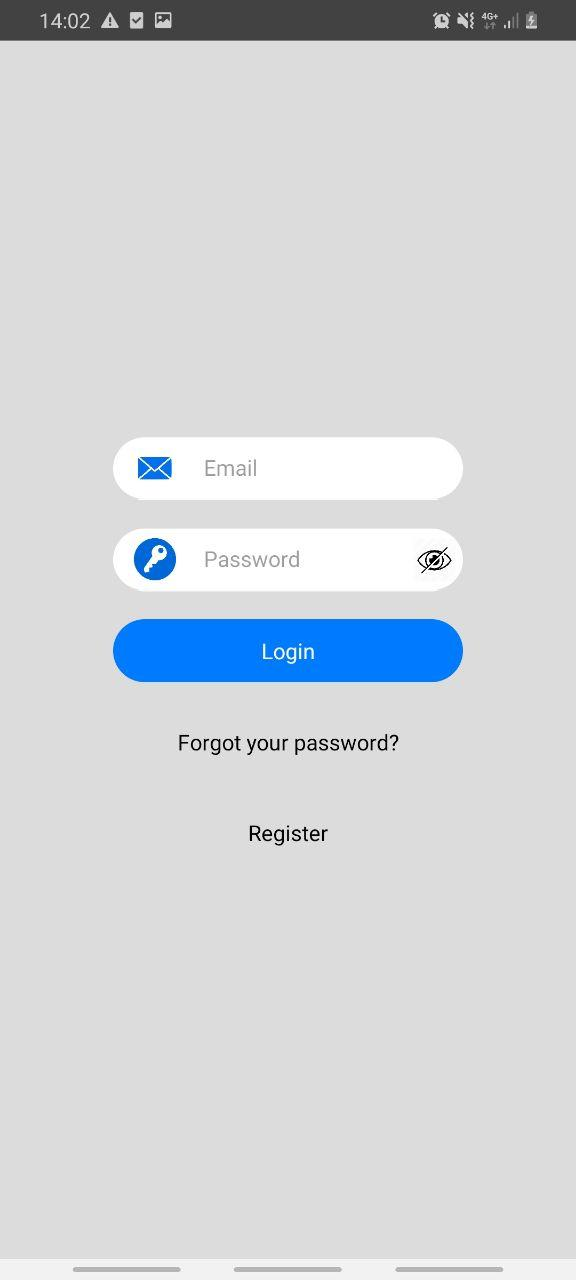
\includegraphics[width=\linewidth,keepaspectratio=true]{img/register.jpg}
\caption{Login Page}
\label{fig:Login}
\end{minipage}
\end{figure}


\begin{figure}[ht]
    \centering
    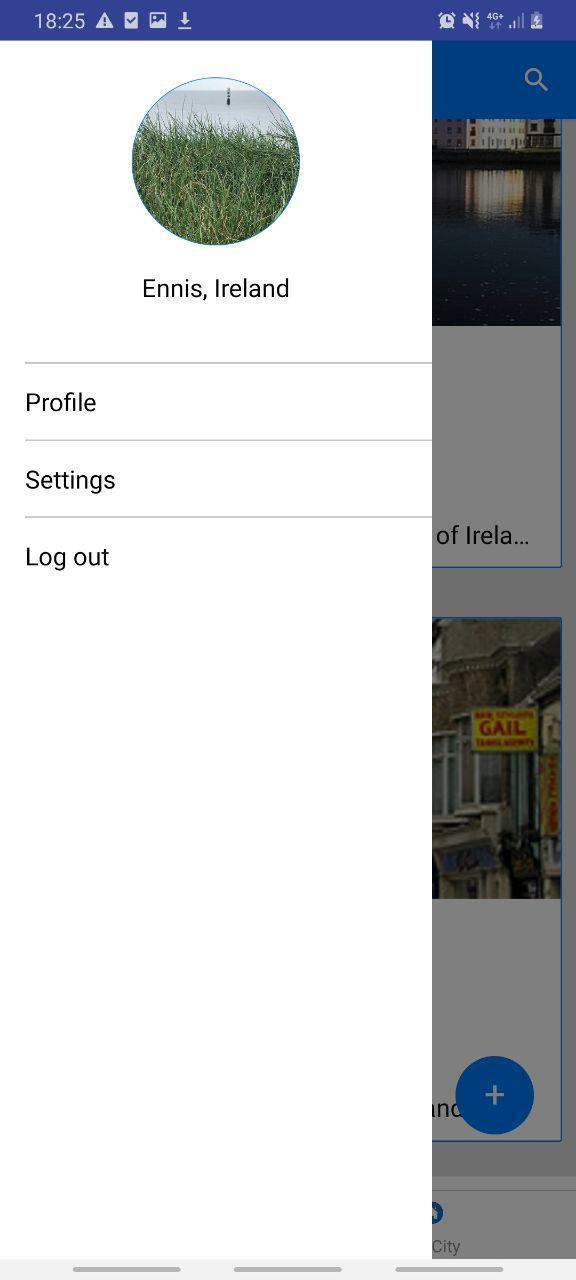
\includegraphics[width=0.5\textwidth]{img/drawer.jpg}
     \caption{Drawer}
    \label{fig:Drawer}
\end{figure}


\begin{figure}[h!]
\begin{minipage}[t]{0.48\textwidth}

\includegraphics[width=\linewidth,keepaspectratio=true]{img/profile1.jpg}
\caption{Profile }
\label{fig:Profile}
\end{minipage}
\hspace*{\fill} % it's important not to leave blank lines before and after this command
\begin{minipage}[t]{0.48\textwidth}
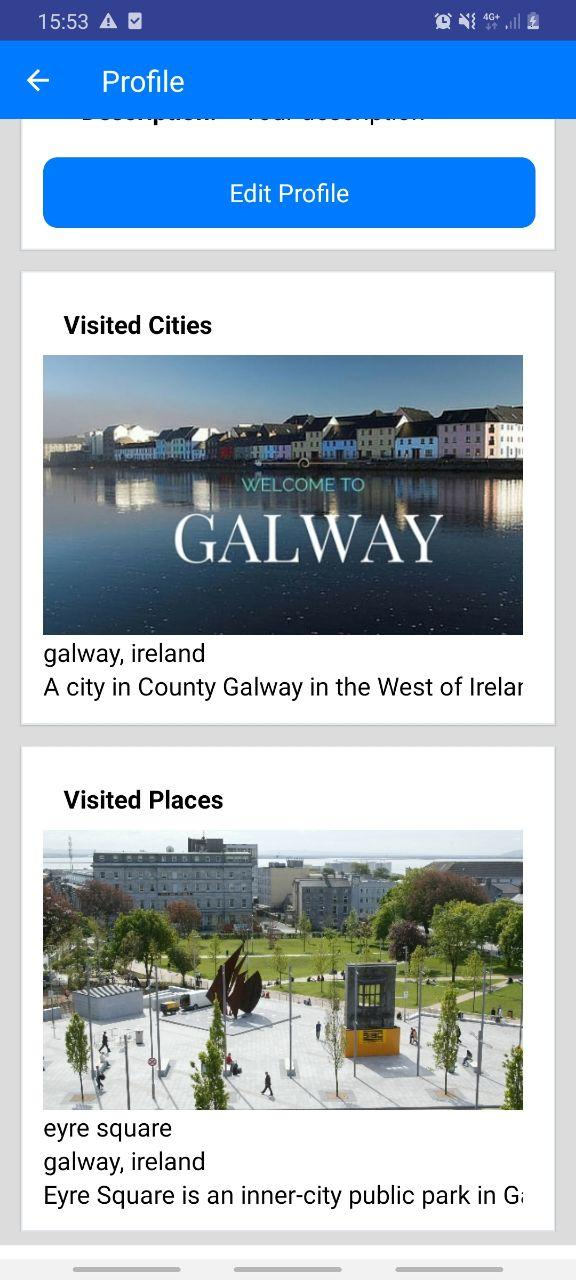
\includegraphics[width=\linewidth,keepaspectratio=true]{img/profile2.jpg}
\caption{Profile cont.}
\label{fig:Profile2}
\end{minipage}
\end{figure}


\begin{figure}[h!]
\begin{minipage}[t]{0.48\textwidth}
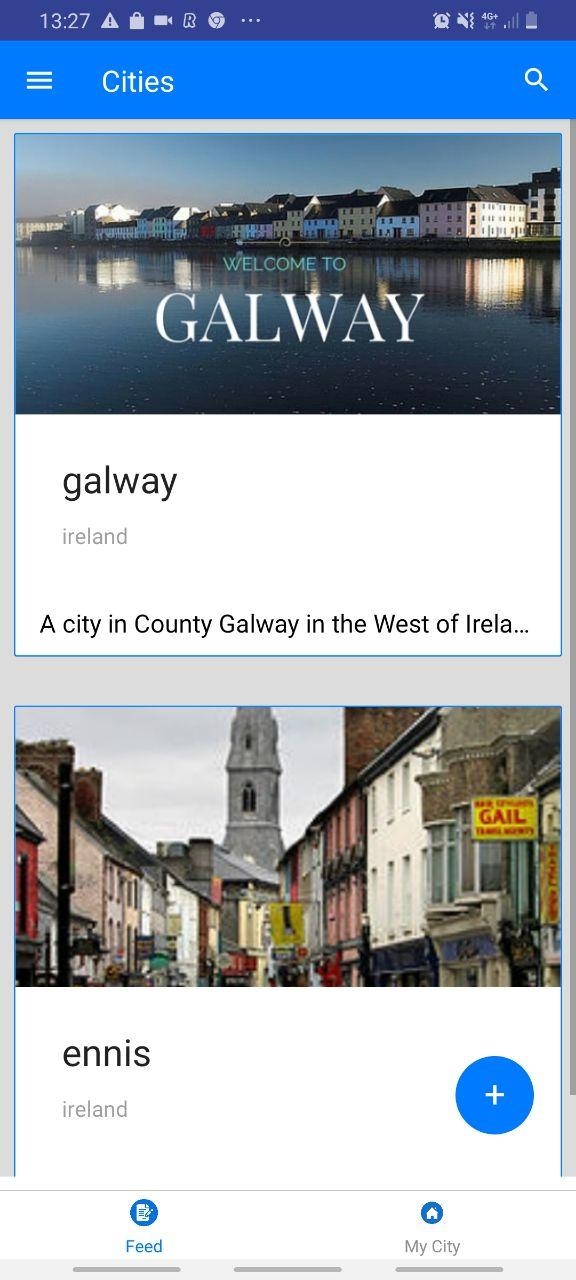
\includegraphics[width=\linewidth,keepaspectratio=true]{img/home_page.jpg}
\caption{Feed}
\label{fig:Feed}
\end{minipage}
\hspace*{\fill} % it's important not to leave blank lines before and after this command
\begin{minipage}[t]{0.48\textwidth}
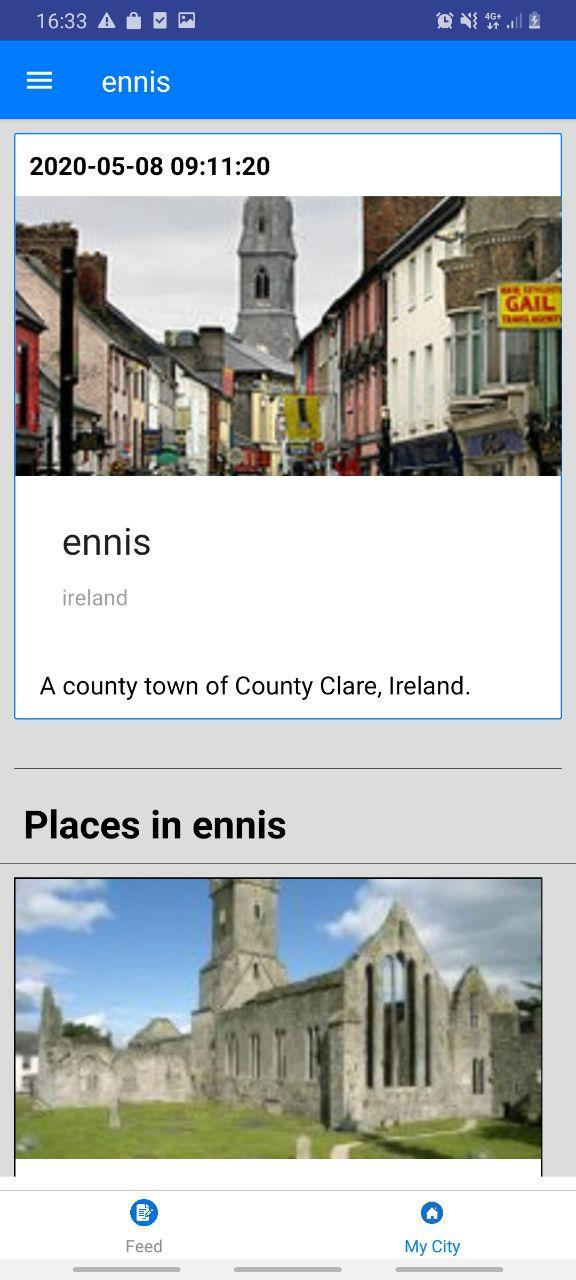
\includegraphics[width=\linewidth,keepaspectratio=true]{img/mycity.jpg}
\caption{My City}
\label{fig:My City}
\end{minipage}
\end{figure}

% ---------------------------------------------------------------
% Steps to Create City

\begin{figure}[h!]
\begin{minipage}[t]{0.48\textwidth}
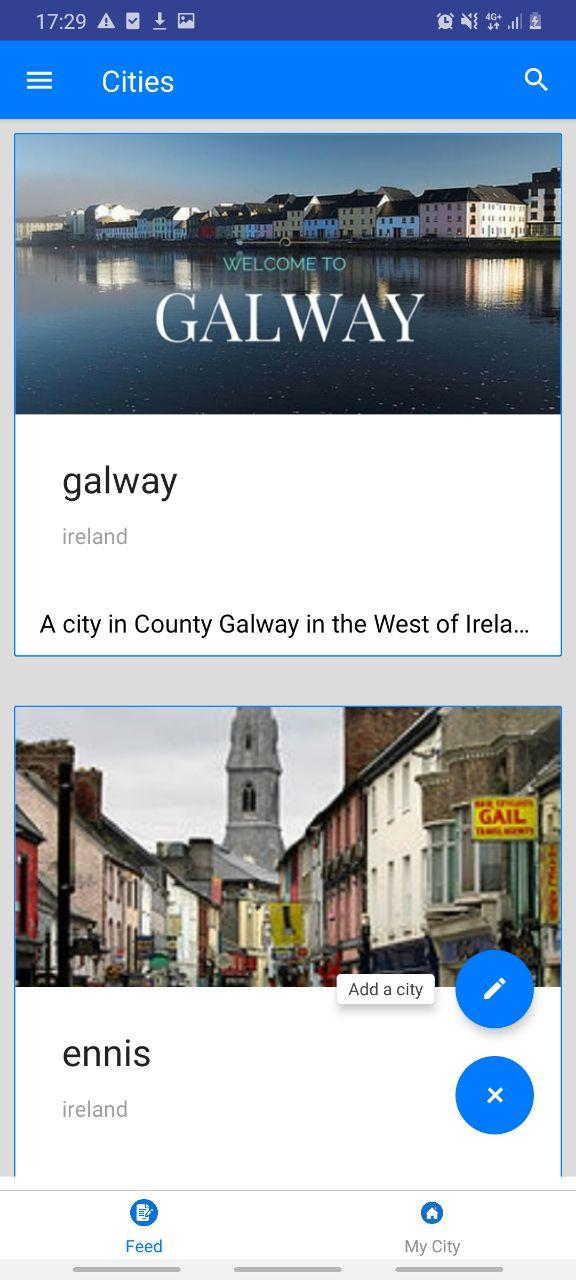
\includegraphics[width=\linewidth,keepaspectratio=true]{img/add_city.jpg}
\caption{Create City Step 1}
\label{fig:Create City}
\end{minipage}
\hspace*{\fill} % it's important not to leave blank lines before and after this command
\begin{minipage}[t]{0.48\textwidth}
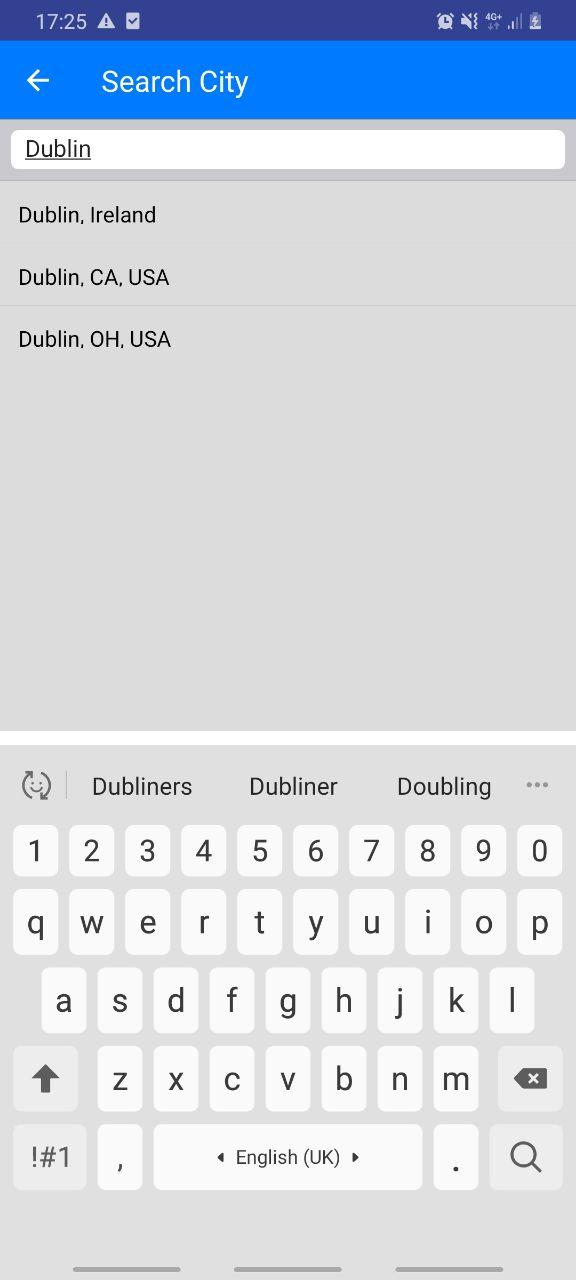
\includegraphics[width=\linewidth,keepaspectratio=true]{img/search.jpg}
\caption{Create City Step 2}
\label{fig:Create City2}
\end{minipage}
\end{figure}

\begin{figure}[h!]
\begin{minipage}[t]{0.48\textwidth}
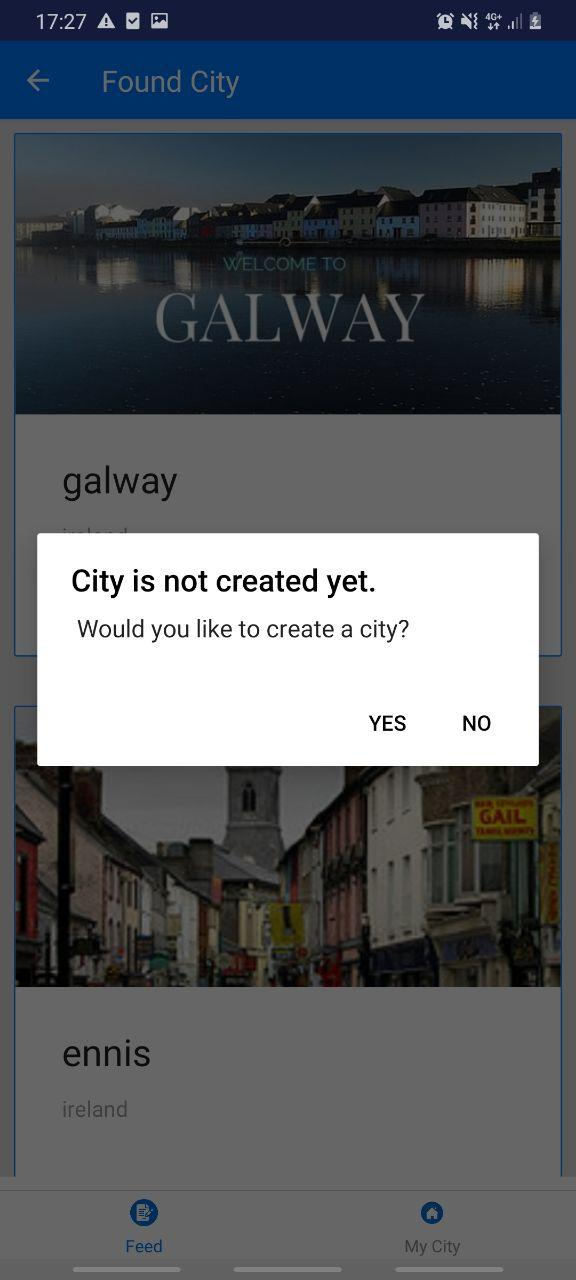
\includegraphics[width=\linewidth,keepaspectratio=true]{img/city_is_not_created.jpg}
\caption{fig:Create City Step 3}
\label{Create City3}
\end{minipage}
\hspace*{\fill} % it's important not to leave blank lines before and after this command
\begin{minipage}[t]{0.48\textwidth}
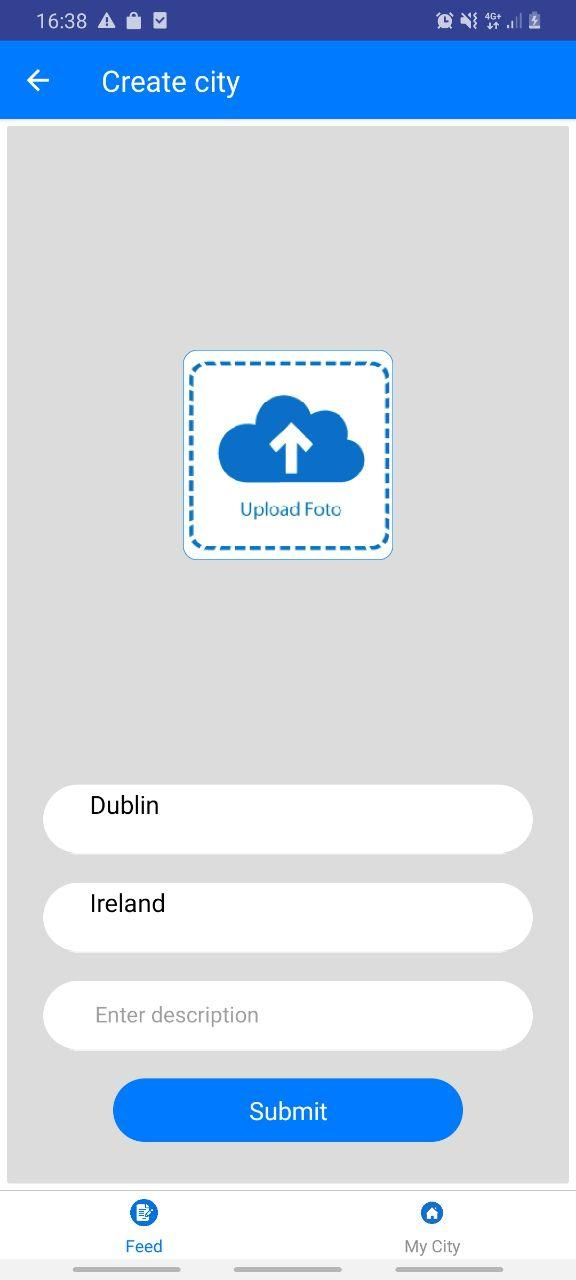
\includegraphics[width=\linewidth,keepaspectratio=true]{img/createCity.jpg}
\caption{Create City Step 4}
\label{fig:Create City4}
\end{minipage}
\end{figure}

\begin{figure}[h!]
\begin{minipage}[t]{0.48\textwidth}
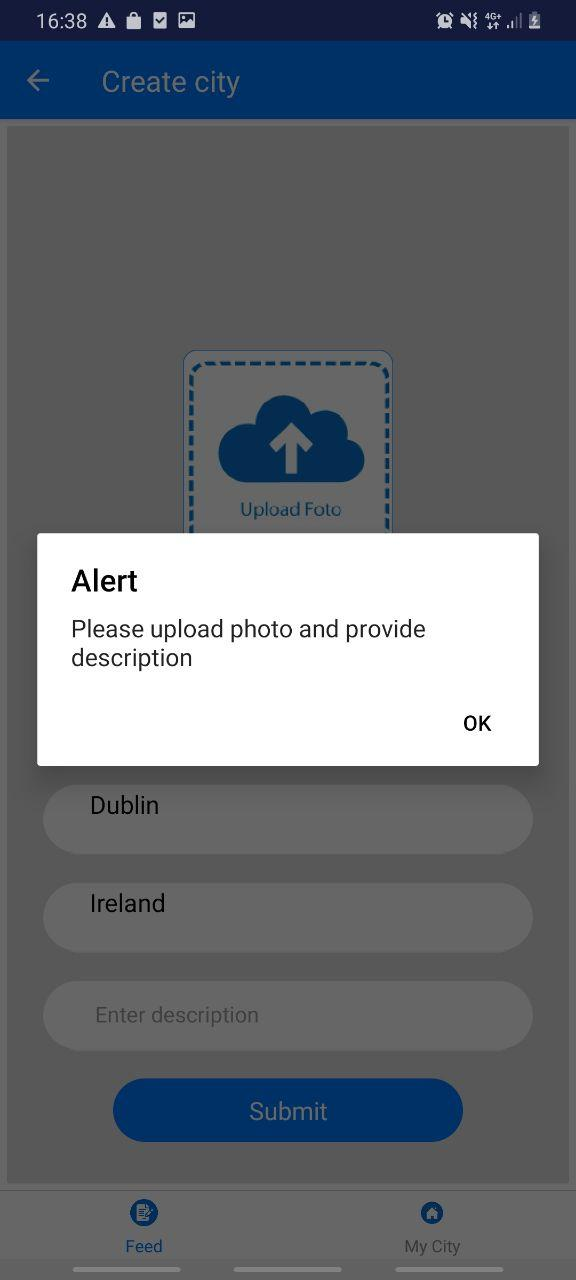
\includegraphics[width=\linewidth,keepaspectratio=true]{img/alert.jpg}
\caption{Create City Step 5}
\label{fig:Create City5}
\end{minipage}
\hspace*{\fill} % it's important not to leave blank lines before and after this command
\begin{minipage}[t]{0.48\textwidth}
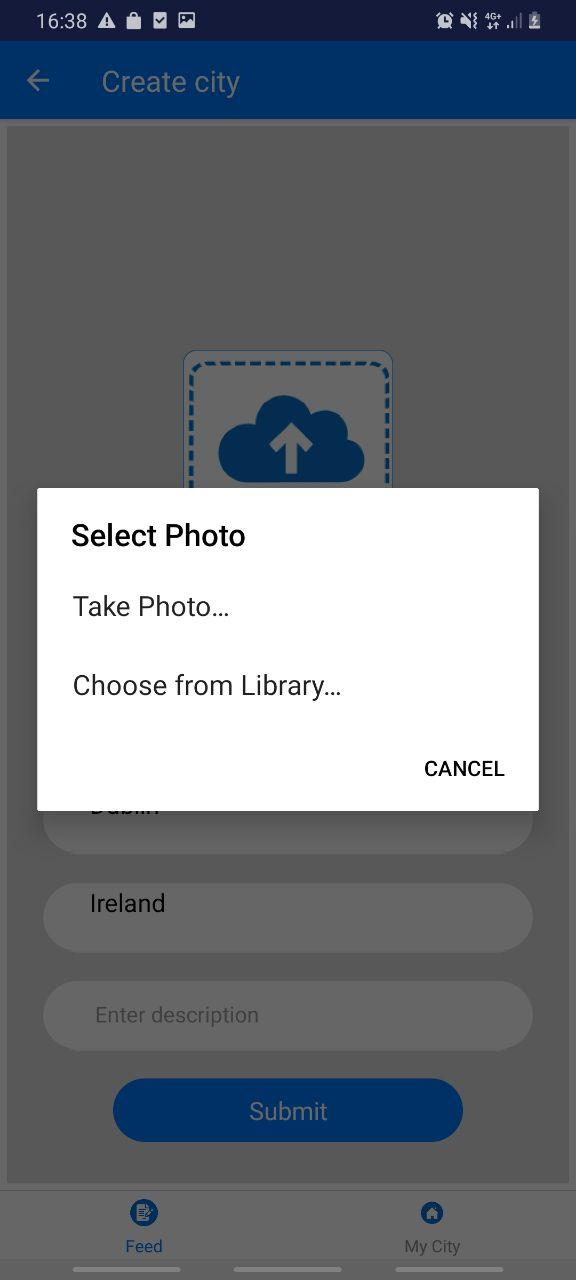
\includegraphics[width=\linewidth,keepaspectratio=true]{img/uploadPhoto.jpg}
\caption{Create City Step 6}
\label{fig:Create City6}
\end{minipage}
\end{figure}


% ------------------------------------------------------------
% Posts about a Place

\begin{figure}[h!]
\begin{minipage}[t]{0.48\textwidth}
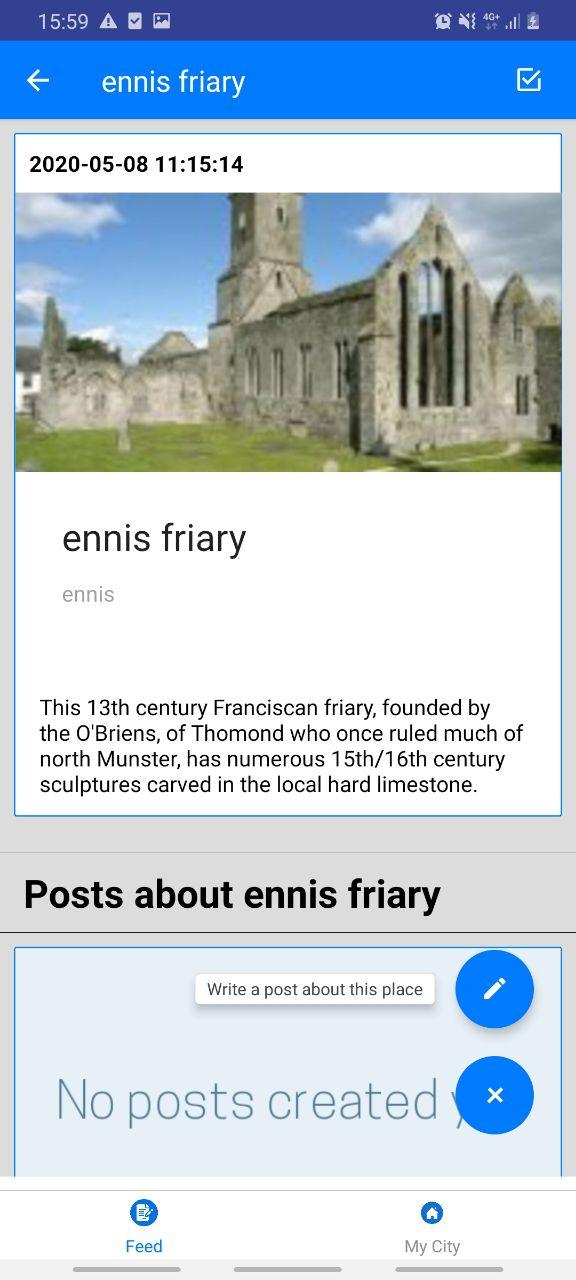
\includegraphics[width=\linewidth,keepaspectratio=true]{img/placeDetails.jpg}
\caption{Place Post}
\label{Place Post}
\end{minipage}
\hspace*{\fill} % it's important not to leave blank lines before and after this command
\begin{minipage}[t]{0.48\textwidth}
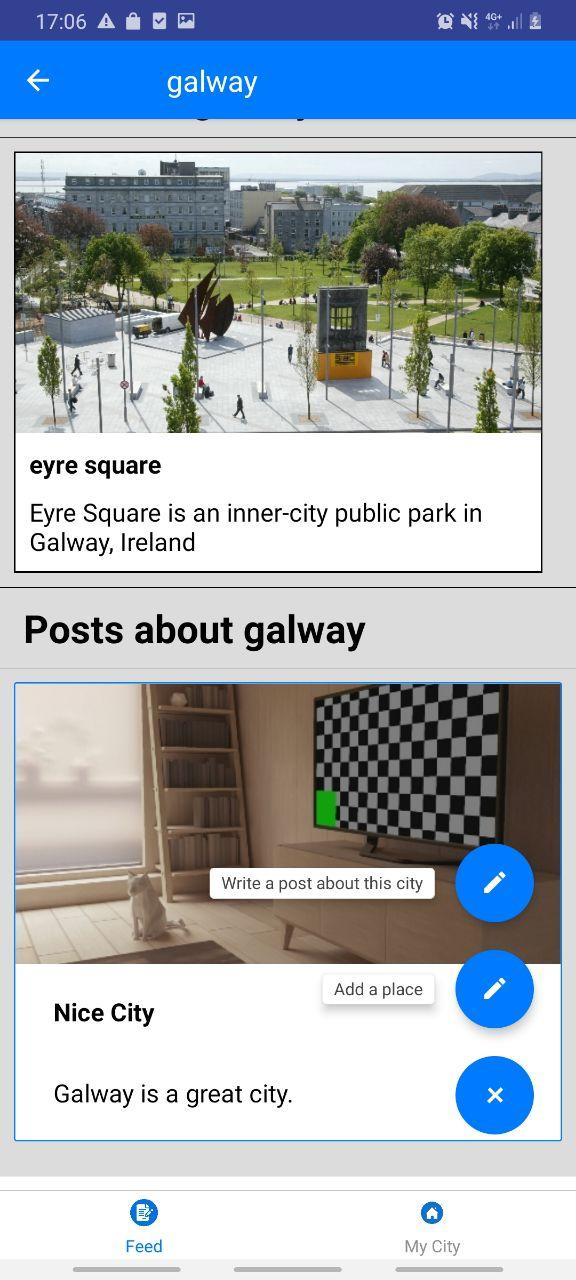
\includegraphics[width=\linewidth,keepaspectratio=true]{img/posts.jpg}
\caption{Post added}
\label{fig:Post Added}
\end{minipage}
\end{figure}





